\documentclass{beamer}

\usepackage{beamerthemeblackboard}
\usepackage{graphics}

\begin{document}

% set handwritten font, necessary packages are loaded in beamerthemeblackboard.sty
%\ECFAugie

\begin{frame}
\title{Mariokart \\ An autonomous go-kart}
\author{Henry Jenkins}
\date{September 26, 2011}
\institute[2011]{Department of Computer and Electrical Engineering,\\
    University of Canterbury, \\ Christchurch, \\ New Zealand}
\maketitle
\end{frame}

\begin{frame}
\frametitle{Overview}
The Goal
\begin{itemize}
\item ``The aim of this project is to take the departments go-karts and build in a
system to replace the human driver. This will entail (at least), selection of
appropriate actuators, motion and distance sensors, development of a navigation
system, an interface to the existing control system, and a central computing
platform. A suitable navigational goal would include a circumnavigation of S
block.''
\end{itemize}

Our Goal
\begin{itemize}
\item Make a robust platform for future projects
\item Set sub-goal of of drive-by-wire go-kart
\end{itemize}
\end{frame}

\begin{frame}
\frametitle{Hardware Layout}
\framesubtitle{asd}
\end{frame}

\begin{frame}
\frametitle{Hardware Layout}
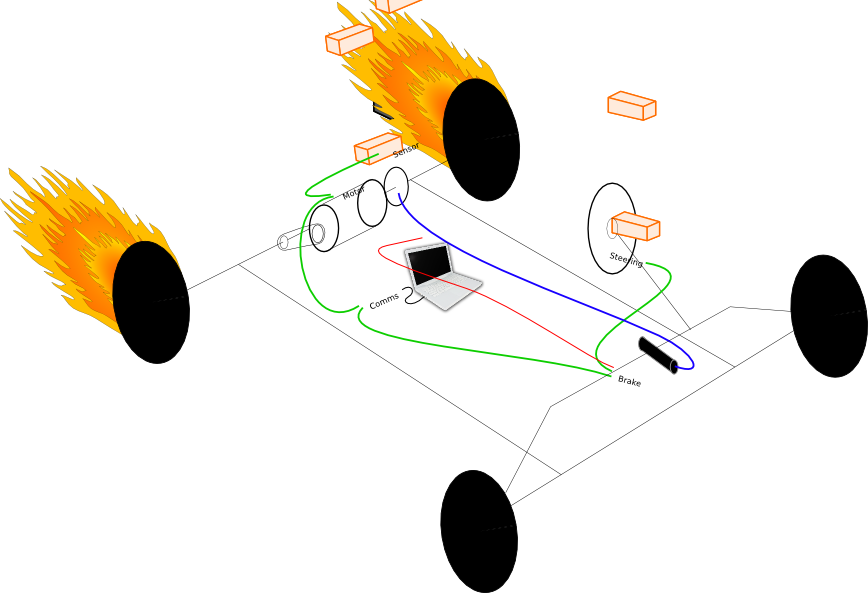
\includegraphics{../../hardware_layout/layout.png}
\end{frame}

\begin{frame}
\frametitle{How it all communicates}
\framesubtitle{asd}
\end{frame}

\begin{frame}
\frametitle{Project time line}
\framesubtitle{asd}
\end{frame}

\begin{frame}
\frametitle{Conclusion}
\framesubtitle{asd}
\begin{itemize}
\item Only 3 mistakes on boards
\item Nice hardware platform for future years
\item Expandable hardware
\begin{itemize}
\item 2 x SPI ports
\item 5v
\item Sweet Project
\end{itemize}
\end{itemize}
\end{frame}

\end{document}
